\section{BPMN-models}
	The following BPMN-models\cite{bpmn} describe how we view the current processes of registering to a course, and complaining on a grade, followed by our suggested changes.
All models are from a student's perspective, as that is what we found most interesting.

\subsection{Registering to a course}
	As shown in figure \ref{fig:Register-old}, the current process of selecting courses, and registering to them, is very cumbersome for the students.
The information about each course is spread around on different sites, and due to It's Learning being used to handle all information released during a semester,
there is no simple way for students to see what a course actually contains.

Figure \ref{fig:Register-new} shows our suggested changes to this process.
With all information gathered at a single site, we can offer students a coherent experience and improved functionality.
The students can follow the old approach, and manually look through courses, log in at the end, and register,
or they can at any earlier point chose to log in and utilize the course suggestion feature to simplify selection.
\begin{figure}[H]
    \centering
    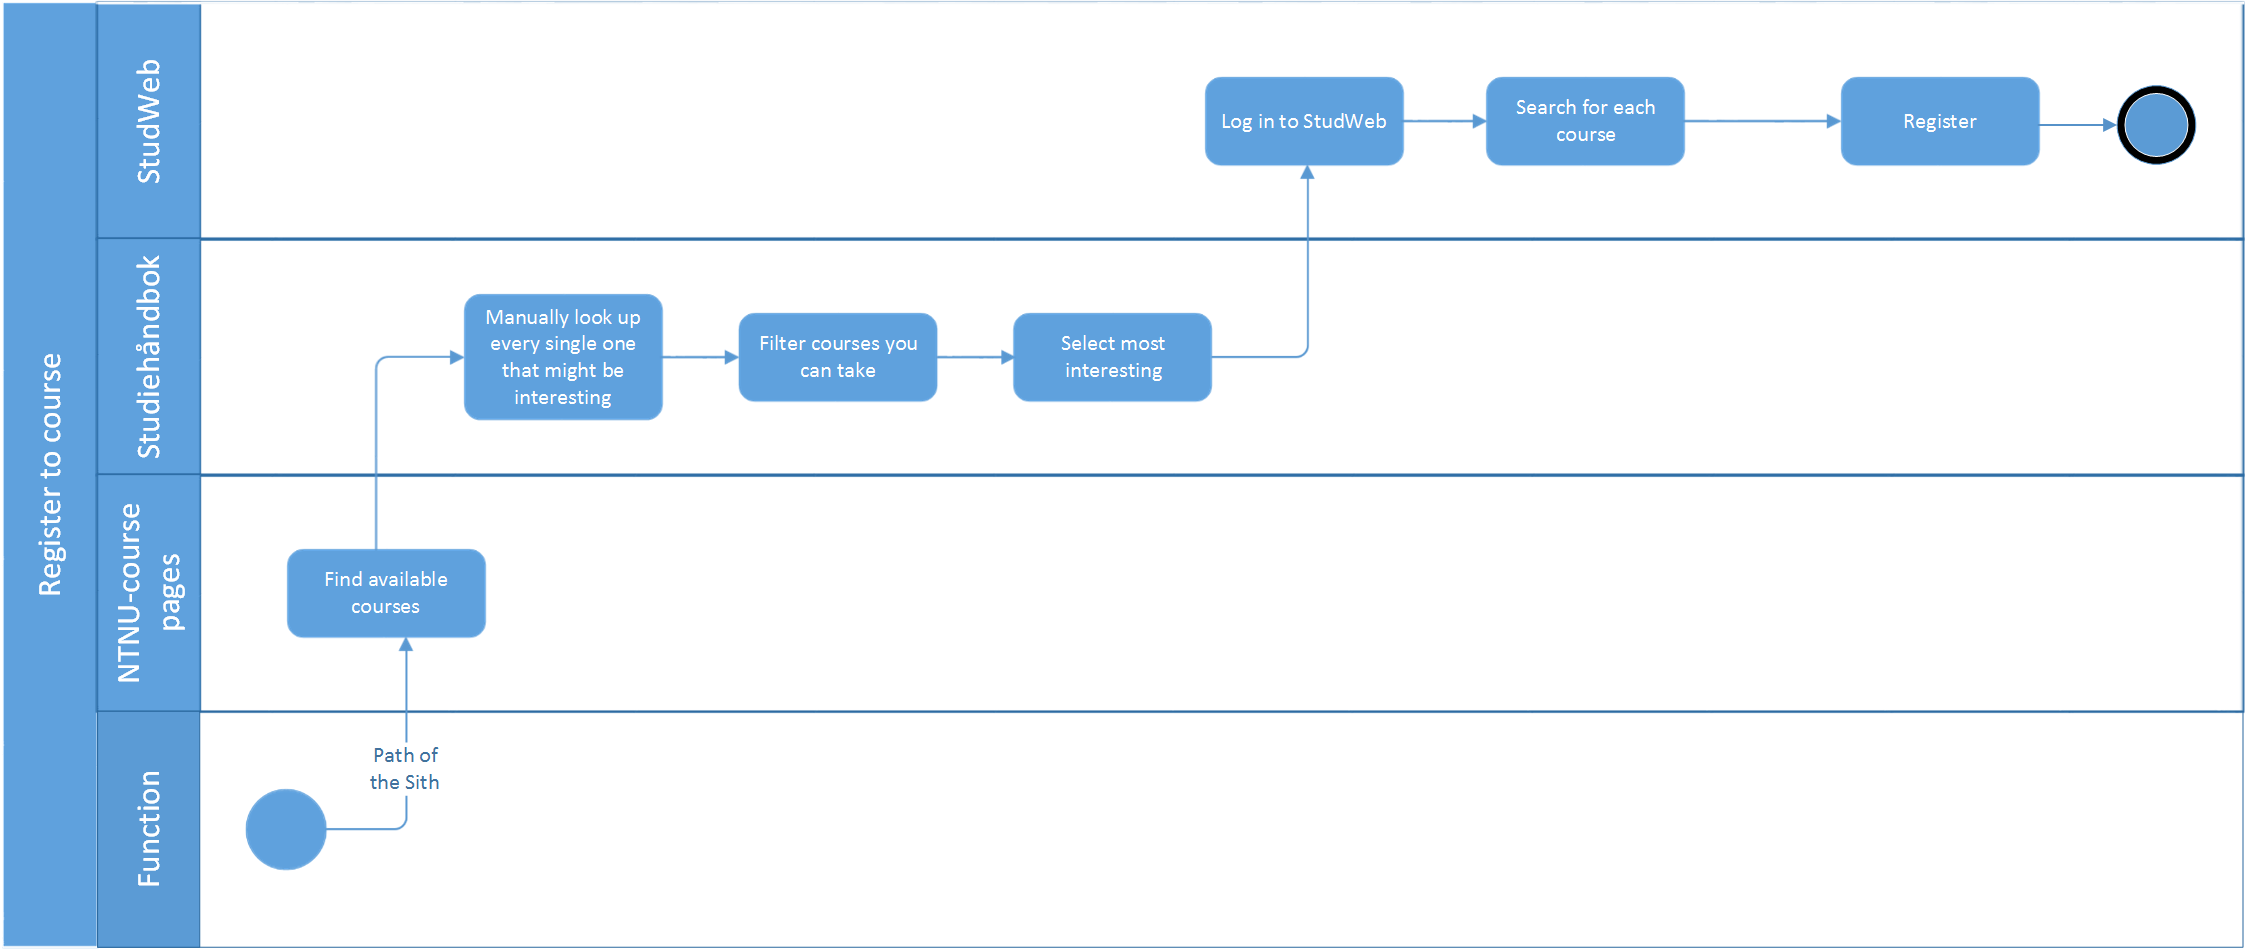
\includegraphics[width=\textheight, angle=-90]{BPMN-register-old}%apparently sets width first and then rotates
    \caption{Our interpretation of the current process of registering to a course.}
    \label{fig:Register-old}
\end{figure}

\begin{figure}[H]
    \centering
    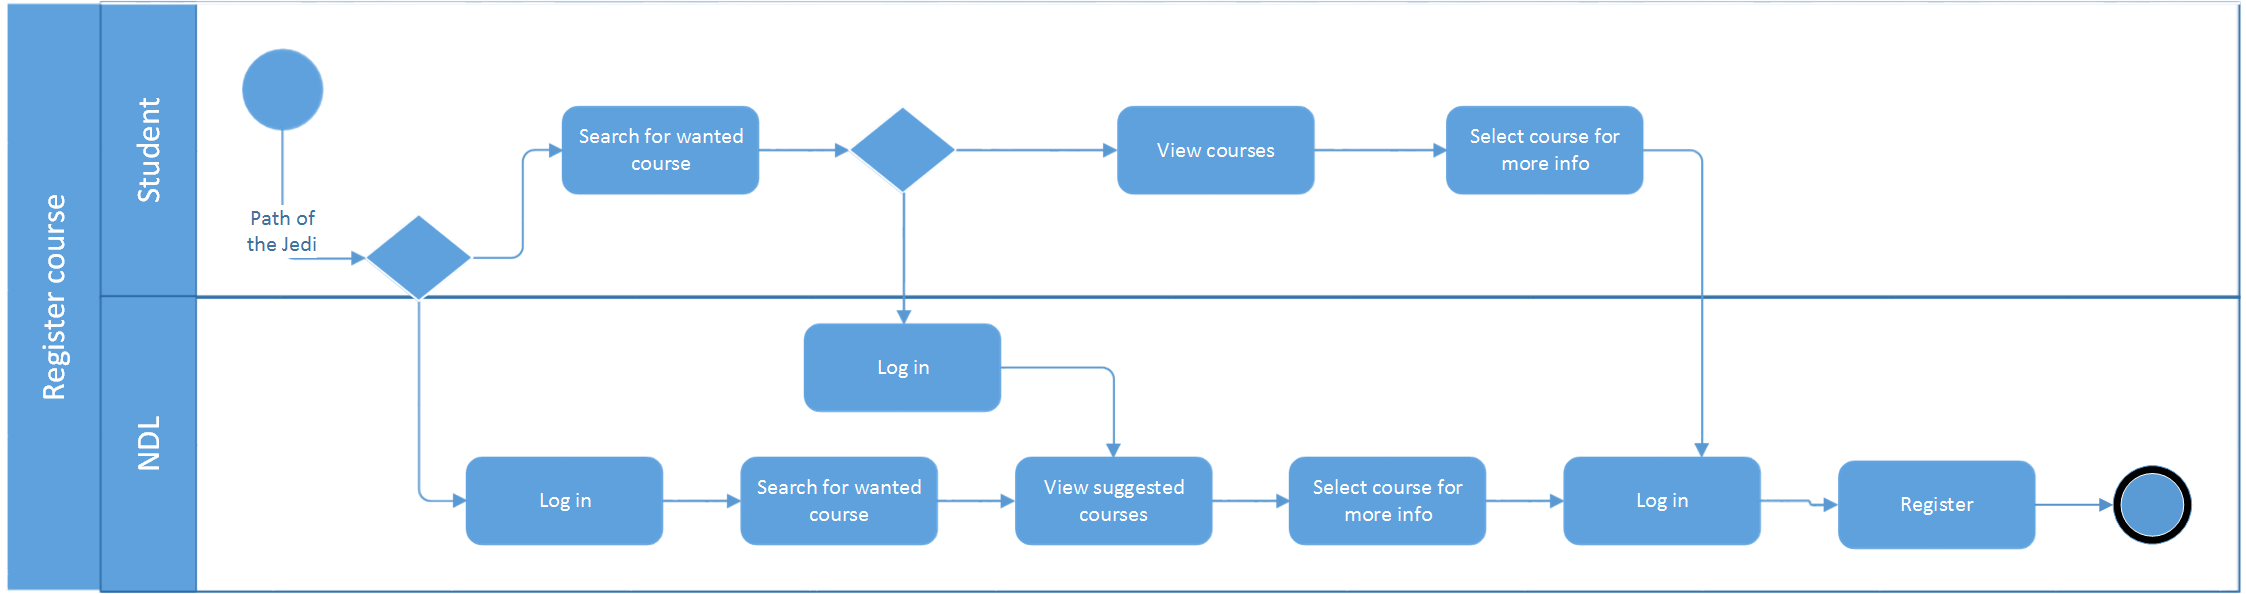
\includegraphics[width=\textheight, angle=-90]{BPMN-register}
    \caption{How we envision our new process of registering to a course to be.}
    \label{fig:Register-new}
\end{figure}

\subsection{Complaining on a grade}
	

\begin{figure}[H]
    \centering
    \includegraphics[width=\textheight, angle=-90]{BPMN-complain-old}
    \caption{Our interpretation of the current process of complaining on a grade.}
    \label{fig:Complain-old}
\end{figure}

\begin{figure}[H]
    \centering
    \includegraphics[width=\textheight, angle=-90]{BPMN-complain}
    \caption{How we envision our new process of complaining to be.}
    \label{fig:Complain-new}
\end{figure}
